\section{Strukturorientierte Testverfahren}

\begin{tcolorbox}
    Bei \textbf{strukturorientierten Testverfahren}, auch \textbf{White-Box-Tests} genannt, wird zur \textbf{Konstruktion der Testfälle} als auch zur \textbf{Bestimmung der Vollständigkeit} der Tests der Quellcode herangezogen.\\
    Dadurch soll sichergestellt werden, dass jede existierende Codezeile in Tests ausgeführt worden ist.
\end{tcolorbox}


\subsection*{Überdeckungsverfahren}

\begin{tcolorbox}[title=Anweisungsüberdeckung]
    Liegt eine \textbf{Anweisungsüberdeckung} vor, wurde im Test \textit{jede} Anweisung mindestens einmal ausgeführt: \textit{Jeder} Knoten eines \textbf{Kontrollflussgraphen} wurde dann mindestens einmal ausgeführt.
\end{tcolorbox}

\begin{tcolorbox}[title=Zweigüberdeckung]
    Eine \textbf{Zweigüberdeckung} liegt vor, wenn \textit{jede Kante} des Kontrollflussgraphen mindestens einmal ausgeführt worden ist.
    Es ist also nicht notwendig, alle Bedingungen auf einmal zu erfüllen, solange mit entsprechenden Testdaten jeweils ein Zweig durchlaufen werden kann, und am Ende alle Zweige durchlaufen worden sind.
    \begin{minted}[fontsize=\small]{java}
        // a = 1 -> erstes if
        // a = -2 -> zweites if
        if (a > 0) {...}
        if (a % 2 == 0) {...}
    \end{minted}
    Liegt eine Zweigüberdeckung vor, ist gleichzeitig auch die \textbf{Anweisungsüberdeckung} erfüllt.\\
    Die Zweigüberdeckung bietet schon eine ziemlich vollständige Überdeckung, berücksichtigt aber Schleifen nicht genügend.
\end{tcolorbox}

\begin{tcolorbox}[title=Boundary-Interior-Coverage]
    Das Verhalten des Testgegenstandes beim abweisenden Fall oder bei mehreren Durchläufen einer Schleife führen zu der Forderung der Verallgemeinerung der Möglichkeiten: Im Test sollen alle \textit{Pfade}, die durch den Kontrolflussgraphen laufen, vorkommen.\\
    In diesem Fall spricht man von \textbf{Pfadüberdeckung} (\textit{path coverage} bzw. \textit{loop coverage}).
    Die \textbf{Boundary-Interior-Coverage} ist eine Form der \textbf{Pfadüberdeckung}, bei der bei Schleifen der abweisende Fall (\textit{boundary}) und mindestens zwei Durchläufe (\textit{interior}) genügen.\\
    Wird eine Boundary-Interior-Überdeckung erreicht, ist automatisch auch die \textbf{Zweigüberdeckung} erreicht.
\end{tcolorbox}

\begin{tcolorbox}[title=Einfache Mehrfachbedingungsüberdeckung]
    Die \textbf{einfache Mehrfachbedingungsüberdeckung} wird erreicht, wenn \textit{jede} atomare Bedingung, also jeder \textit{direkte Vergleich}, und \textit{alle zusammengesetzten Bedingungen} einmal den Wahrheitswert \textit{wahr} und einmal den Wahrheitswert \textit{falsch} annehmen\footnote{
        \textit{Maxterm}: Für genau eine Variablenbelegung falsch (Disjunktion: $A \lor B \lor C$); bzw. \textit{Minterm}: für genau eine Variablenbelegung wahr (Konjunktion: $A \land B \land C$)(vgl.~\cite[92]{Hof22})
    }.\\
    Dadurch wird gleichzeitig eine \textbf{Zweigüberdeckung} erreicht
\end{tcolorbox}

\begin{figure}
    \centering
    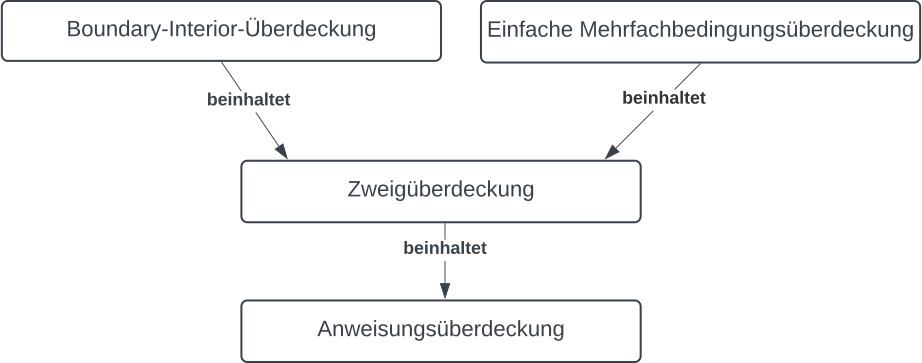
\includegraphics[scale=0.4]{part four/Testende Verfahren/img/coverage-criteria-hierarchy}
    \caption{Hierarchie der verschiedenen Überdeckungskriterien. (Quelle: in Anlehnung an \cite[Abb. 5.2, 53]{Wed09c})}
    \label{fig:coverage-criteria-hierarchy-cc}
\end{figure}